\section{Lọc ảnh trong miền tần số}
Đối với mỗi bức ảnh, những ảnh có tần số thấp là ảnh có sự thay đổi mức xám ít, ví dụ như ảnh một bức tường, mặt biển,... hay ảnh có tần số cao khi thay đổi mức xám đột ngột như biên của vật thể. Vì vậy, trong nhiều trường hợp ta cần có bộ lọc $H(u,v)$ thể làm giảm đi tần số cao trong khi đi qua các tần số thấp (gọi là lọc thông thấp) làm cho ảnh mờ đi, hay bộ lọc có tính chất ngược với lọc thông thấp (gọi là lọc thông cao) giúp tăng cường chi tiết hình dạng vật thể, đồng thời tăng độ tương phản ảnh. Đồ án sẽ đề cập đến các bộ lọc và ứng dụng của chúng.
%\begin{itemize}
%    \item Lọc thông thấp Ideal (Ideal low pass filter)
%    \item Lọc thông thấp Gaussian (Gaussian low pass filter)
%    \item Lọc thông thấp Butterworth (Butterworth low pass filter)
%    \item Lọc thông cao Ideal (Ideal high pass filter)
%    \item Lọc thông cao Gaussian (Gaussian high pass filter)
%    \item Lọc thông cao Butterworth (Butterworth high pass filter)
%\end{itemize}
\subsection{Lọc thông thấp}
\par Lọc thông thấp Ideal:
$$H(u,v) = \left\{ {\begin{array}{*{20}{c}}
{1\,\,\,\,if\,D(u,v)\, \le \,{D_0}}\\
{0\,\,\,\,if\,D(u,v)\, > \,{D_0}.}
\end{array}} \right.$$
Lọc thông thấp Gaussian:
%$$G(x,y) = \frac{1}{{2\pi {\sigma ^2}}}{e^{ - {\textstyle{{{x^2} + {y^2}} \over %{2{\sigma ^2}}}}}}$$

%Như vậy, ta có công thức của bộ lọc Gaussian:
$$H(u,v) = \frac{1}{{2\pi {\sigma ^2}}}{e^{ - {\textstyle{{{D^2}(u,v)} \over {2{\sigma ^2}}}}}}.$$
Lọc thông thấp Butterworth
$$H(u,v) = \frac{1}{{1 + {{\left[ {\frac{{D(u,v)}}{{{D_0}}}} \right]}^{2n}}}}$$
\\
trong đó $D_0$ là hằng số dương và $D(u,v)$ là khoảng cách giữa điểm $(u,v)$ trong miền tần số và tâm của hình chữ nhật tần số, tức là:
$$D(u,v) = \sqrt {{{(u - \frac{{\rm{W}}}{2})}^2} + {{(v - \frac{{\rm{H}}}{2})}^2}} $$
hoặc công thức đã được chuẩn hóa:
$$D(u,v) = \sqrt {{{(0.5 - \frac{u}{{\rm{W}}})}^2} + {{(0.5 - \frac{v}{H})}^2}} $$
với W, H lần lượt là chiều dài và chiều rộng của bức ảnh, $\sigma$ là độ lệch chuẩn trong hàm Gaussian và $n$ là cấp của bộ lọc Butterworth.
\begin{center}
    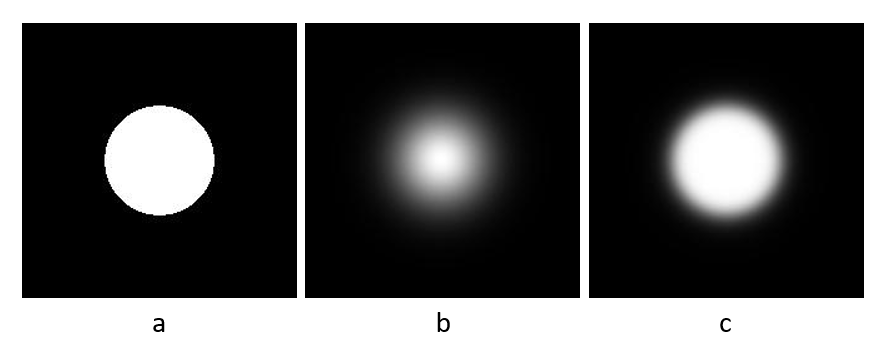
\includegraphics[scale=0.55]{Figures/fig6.png}
    \par \textbf {Hình 2.1} Bộ lọc thông thấp (a: Ideal, b: Gaussian, c: Butterworth).
\end{center}
\par Ảnh đầu vào sau khi thông qua biến đổi Fourier sẽ được nhân pixel-by-pixel với bộ lọc, kết quả thu được thông qua biến đổi Fourier ngược sẽ là ảnh đã được lọc.
\begin{center}
    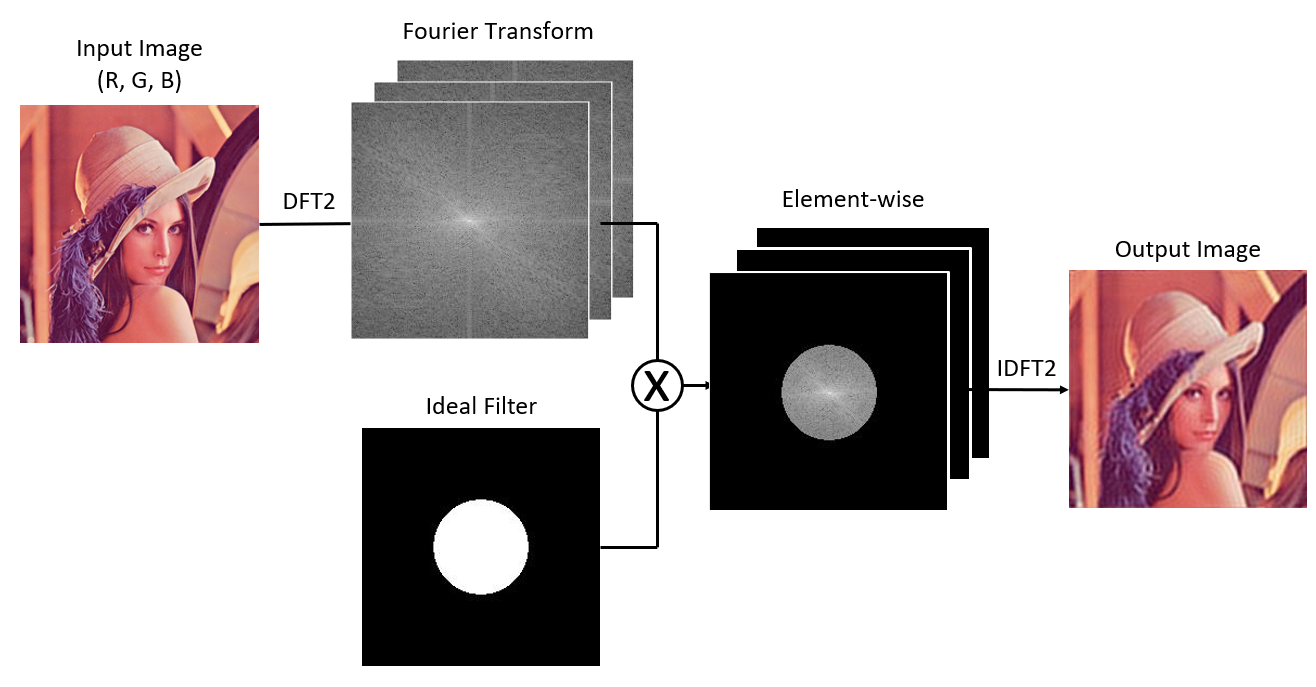
\includegraphics[scale=0.45]{Figures/fig1.png}
    \par \textbf {Hình 2.2} Lọc ảnh màu trong miền tần số bằng bộ lọc thông thấp Ideal.
\end{center}

Ảnh màu được cấu tạo bằng nhiều kênh màu khác nhau, thông dụng nhất là ảnh màu RGB với tương ứng 3 kênh màu Red-Green-Blur. Trong trường hợp muốn áp dụng bộ lọc cho ảnh màu RGB, ta sẽ áp dụng bộ lọc với từng kênh màu, coi mỗi kênh màu là một bức ảnh xám và ảnh thu được sẽ là kết hợp từ các kênh màu đã được lọc (hình 2.2).
\par Mã nguồn cho lọc thông thấp Ideal như sau:

\begin{lstlisting}[language=Matlab]
function filted_img = filterIdealLowPass(img,D0)
    % FFT input image
    fft_img = fftshift(fft2(double(img)));
    % Create low pass Ideal filter
    [H,W,c] = size(img);
    ctx = (W-1)/2;
    cty = (H-1)/2;
    [x, y] = meshgrid(1:W, 1:H);
    mg = sqrt((x - ctx ).^2 + (y - cty).^2);
    filter = double(mg <= D0);
    % Element-wise multiply each channel with the filter
    im = zeros(size(img));
    for z = 1:c
        im(:,:,z) = fft_img(:,:,z) .* filter;
    end 
    % IFFT to get ouput image
    filted_img = ifft2(ifftshift(im));
end
\end{lstlisting}
Bằng việc thay cách tạo bộ lọc, ta có mã nguồn tương ứng cho lọc thông thấp Gaussian và Butterworth.

\begin{lstlisting}[language = Matlab]
function filted_img = filterGaussianLowPass(img,fc)
    % FFT input image
    fft_img = fftshift(fft2(double(img)));
    % Create low pass Gaussian filter
    [H,W,c] = size(img);
    ctx = (W-1)/2;
    cty = (H-1)/2;
    a = 1/(2*pi*sig*sig);
    b = 2*sig*sig;
    [x, y] = meshgrid(1:W, 1:H);
    D2 = (x - ctx ).^2 + (y - cty).^2;
    filter = a*exp(-D2/b);
    filter = filter/max(filter(:))
    % Element-wise multiply each channel with the filter
    im = zeros(size(img));
    for z = 1:c
        im(:,:,z) = fft_img(:,:,z) .* filter;
    end 
    % IFFT to get ouput image
    filted_img = ifft2(ifftshift(im));
end
function filted_img = filterButterworthLowPass(img, D0, n)
    % FFT input image
    fft_img = fftshift(fft2(double(img)));
    % Create low pass Butterworth filter
    [H,W,c] = size(img);
    ctx = (W-1)/2;
    cty = (H-1)/2;
    [x, y] = meshgrid(1:W, 1:H);
    D2 = (x - ctx ).^2 + (y - cty).^2;
    filter = 1./(1+ (D2/D0/D0).^n);
    filter = filter/max(filter(:))
    % Element-wise multiply each channel with the filter
    im = zeros(size(img));
    for z = 1:c
        im(:,:,z) = fft_img(:,:,z) .* filter;
    end 
    % IFFT to get ouput image
    filted_img = ifft2(ifftshift(im));
end
\end{lstlisting}
\par Sau quá trình lọc thông thấp (hình 2.3), ảnh đầu vào sẽ bị giảm các tần số cao, tức là bị làm mờ, độ nét các đường biên giữa vật thể với nền đã bị giảm xuống. Thông qua biểu đồ tần số của bộ lọc Gaussian (hình 2.4), ta có thể thấy sau khi qua bộ lọc biểu đồ trông mượt hơn so với ban đầu. Các tần số của ảnh đã được kéo giãn ra, điều đó có nghĩa là nhiều tần số cao đã được kéo xuống. Tùy vào tính chất của từng bộ lọc mà dẫn đến hiện tượng xuất hiện các đường biên mờ quanh đường biên của vật thể trong ảnh trong bộ lọc Ideal, hay hiện tượng mờ toàn cục của bộ lọc Gaussian. 
\begin{center}
    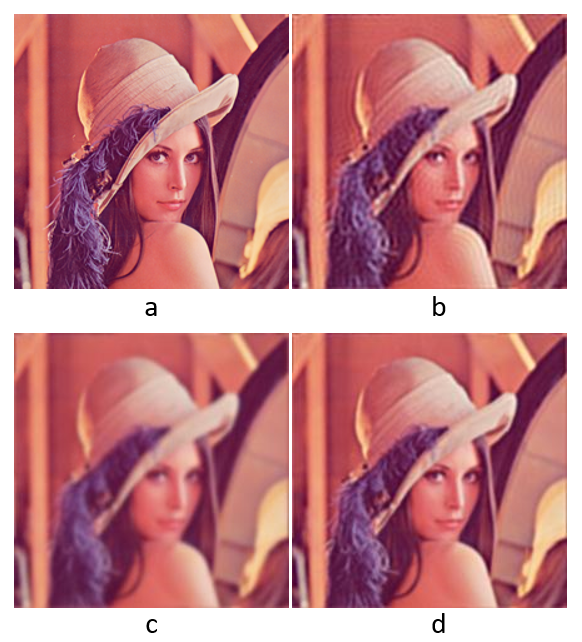
\includegraphics[scale=0.7]{Figures/fig8.png}
    \par \textbf {Hình 2.3} Kết quả sử dụng bộ lọc thông thấp\\ (a: ảnh gốc, b: Ideal, c: Gaussian, d: Butterworth).
\end{center}
\begin{center}
    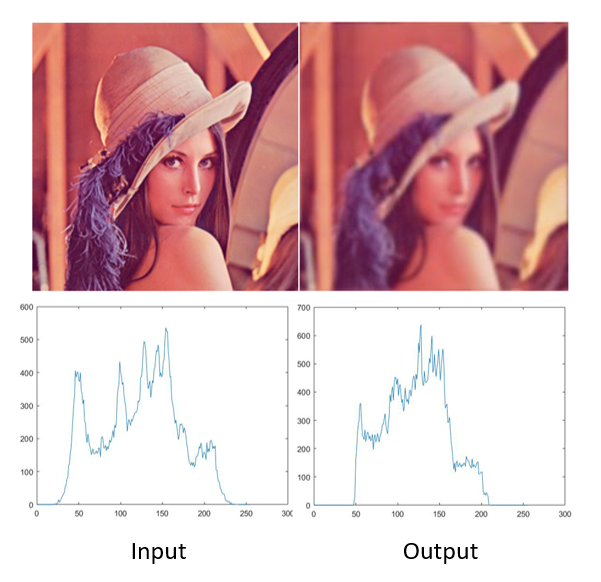
\includegraphics[scale=0.9]{Figures/fig7a.png}
    \par \textbf {Hình 2.4} Lọc thông thấp Gaussian.
\end{center}
\par Phép lọc thông thấp (lọc mờ ảnh) được ứng dụng trong nhận dạng ký tự quang học (OCR), công nghiệp in ấn, xử lý ảnh trên vệ tinh, tăng cường ảnh...

\subsection{Lọc thông cao}
Ngược lại với các bộ lọc thông thấp sẽ là các bộ lọc thông cao. Công thức cơ bản của các bộ lọc thông cao đó là:
$$Hi(u, v) = 1.0 - Lo(u, v)$$
trong đó $Lo(u,v)$ là bộ lọc thông thấp tương ứng mà giá trị mỗi điểm ảnh đã được chuẩn hóa trong đoạn $[0,1]$. Do vậy, ta thu được các bộ lọc như sau:
\begin{center}
    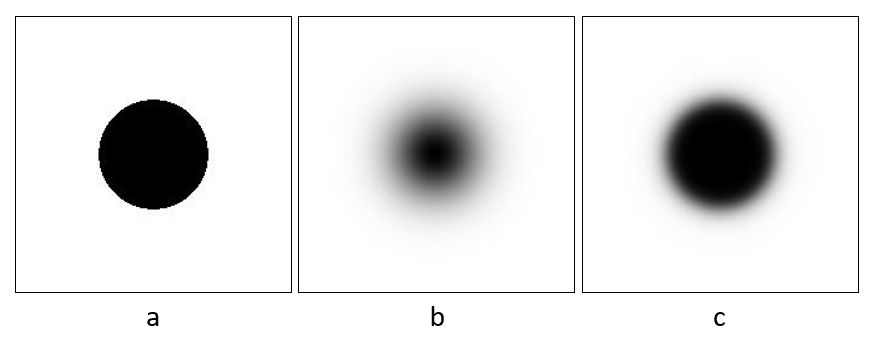
\includegraphics[scale=0.55]{Figures/fig9.png}
    \par \textbf {Hình 2.5} Bộ lọc thông cao (a: Ideal, b: Gaussian, c: Butterworth).
\end{center}
Tương tự như khi thực hiện lọc thông thấp, ta có mã nguồn cho thuật toán lọc thông cao:

\begin{lstlisting}[language=Octave]
function filted_img = filterIdealHighPass(img,D0)
    % FFT input image
    fft_img = fftshift(fft2(double(img)));
    % Create high pass Ideal filter
    [H,W,c] = size(img);
    ctx = (W-1)/2;
    cty = (H-1)/2;
    [x, y] = meshgrid(1:W, 1:H);
    mg = sqrt((x - ctx ).^2 + (y - cty).^2);
    filter = 1.0 - double(mg <= D0);
    % Element-wise multiply 
    im = zeros(size(img));
    for z = 1:c
        im(:,:,z) = fft_img(:,:,z) .* filter;
    end 
    % IFFT to get ouput image
    filted_img = ifft2(ifftshift(im));
end
function filted_img = filterGaussianHighPass(img,fc)
    % FFT input image
    fft_img = fftshift(fft2(double(img)));
    % Create high pass Gaussian filter
    [H,W,c] = size(img);
    ctx = (W-1)/2;
    cty = (H-1)/2;
    a = 1/(2*pi*sig*sig);
    b = 2*sig*sig;
    [x, y] = meshgrid(1:W, 1:H);
    D2 = (x - ctx ).^2 + (y - cty).^2;
    filter = a*exp(-D2/b);
    filter = 1.0 - filter/max(filter(:))
    % Element-wise multiply
    im = zeros(size(img));
    for z = 1:c
        im(:,:,z) = fft_img(:,:,z) .* filter;
    end 
    % IFFT to get ouput image
    filted_img = ifft2(ifftshift(im));
end
function filted_img = filterButterworthHighPass(img, D0, n)
    % FFT input image
    fft_img = fftshift(fft2(double(img)));
    % Create high pass Butterworth filter
    [H,W,c] = size(img);
    ctx = (W-1)/2;
    cty = (H-1)/2;
    [x, y] = meshgrid(-ctx:ctx, -cty:cty);
    D2 = (x/ctx).^2 + (y/cty).^2;
    filter = 1./(1+ (D2/D0/D0).^n);
    filter = 1.0 - filter/max(filter(:))
    % Element-wise multiply
    im = zeros(size(img));
    for z = 1:c
        im(:,:,z) = fft_img(:,:,z) .* filter;
    end 
    % IFFT to get ouput image
    filted_img = ifft2(ifftshift(im));
end
\end{lstlisting}
Để thuận tiện trong việc so sánh, kết quả của lọc thông cao sẽ được thực hiện trên ảnh xám. 
\begin{center}
    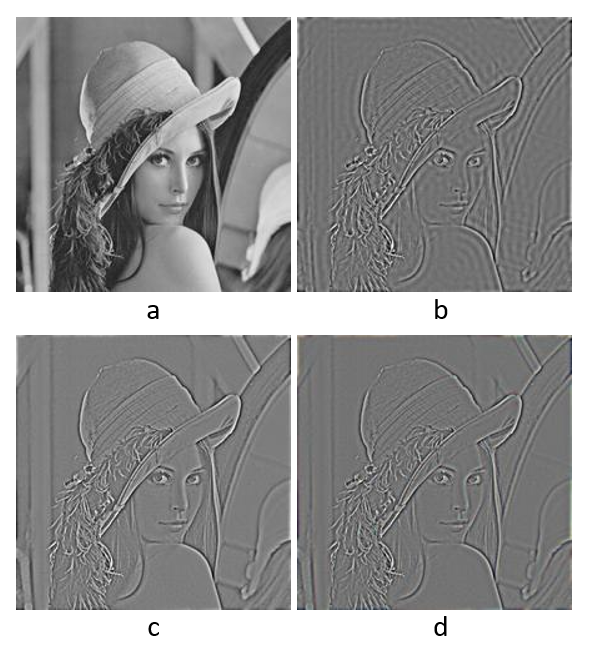
\includegraphics[scale=1.0]{Figures/fig10.png}
    \par \textbf {Hình 2.6} Kết quả sử dụng bộ lọc thông cao\\ (a: ảnh gốc, b: Ideal, c: Gaussian, d: Butterworth).
\end{center}
\par Lọc thông cao được ứng dụng trong việc hỗ trợ và trích xuất các đặc trưng đường, đặc trưng cạnh, làm nổi bật đường biên giữa vật thể và nền.

\section{Tăng cường ảnh}
\subsection{Lọc sắc ảnh dùng trong y tế}
Việc lọc sắc ảnh thường được thực hiện bằng cách cộng có trọng số ảnh gốc với ảnh đã thông qua lọc thông cao (kí hiệu là $HP$)[2]. Bằng cách làm này có thể làm nổi bật đặc trưng đường của ảnh, thông qua đó tăng cường chất lượng của các bộ lọc tiếp theo
$$Sharpen = Original + \lambda * HP$$
trong đó $\lambda$ thường được chọn trong khoảng $(0, 1)$. Mã nguồn của việc lọc sắc nét này như sau:

\begin{lstlisting}[language=Octave]
img = imread('input.jpg');
[H, W, c] = size(img);
img = rgb2gray(img);
weight = 0.5;
% sharpe = get_sharpen(img, 'IDEAL', 0.5);
% sharpe = get_sharpen(img, 'GAUSSIAN', 0.5);
sharpe = get_sharpen(img, 'BUTTERWORTH', 0.5);
function sharpe = get_sharpen(img, method, weight)
    high_pass = abs(get_high_pass(img, method));
    high_pass = mat2gray(high_pass) * 255.0;
    sharpe    = (double(img) + double(high_pass)*weight);
    sharpe    = uint8(sharpe);
end
function high_pass = get_high_pass(img, method)
    if string(method) == 'IDEAL'
        high_pass = IdealHighPass(img, 40);
    elseif string(method) == 'GAUSSIAN'
        high_pass = GaussHighPass(img, 20) ;
    else
        high_pass = ButterworthHighPass(img, 5, 30) ;
    end
end
\end{lstlisting}
Lấy ví dụ đối với bức ảnh chụp lát cắt não bộ và ảnh chụp X-Ray [2], ta thu được kết quả như sau:
\begin{center}
    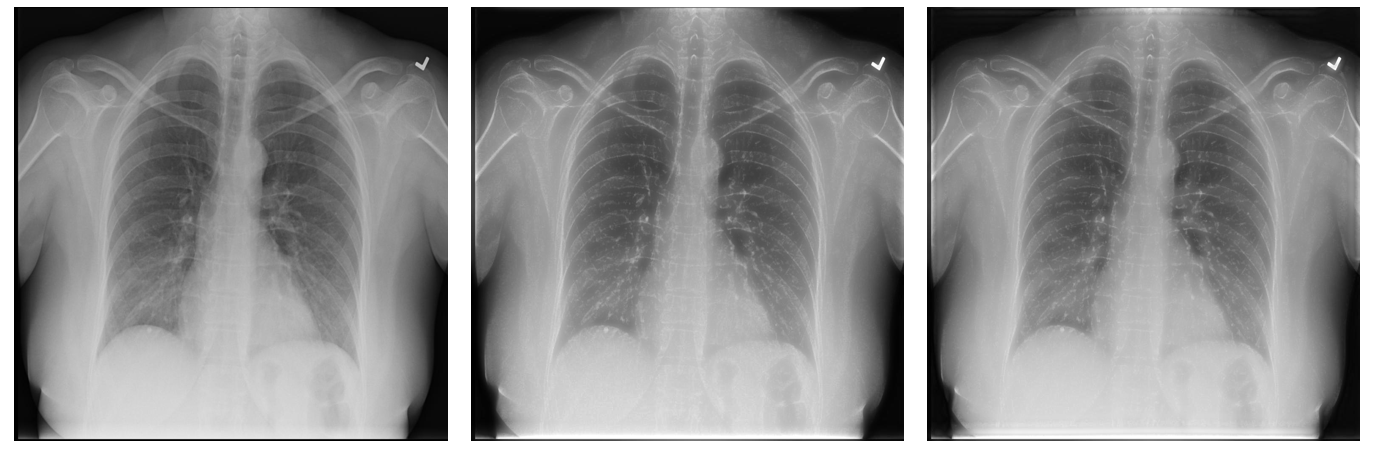
\includegraphics[scale=0.43]{Figures/fig14a.png}
    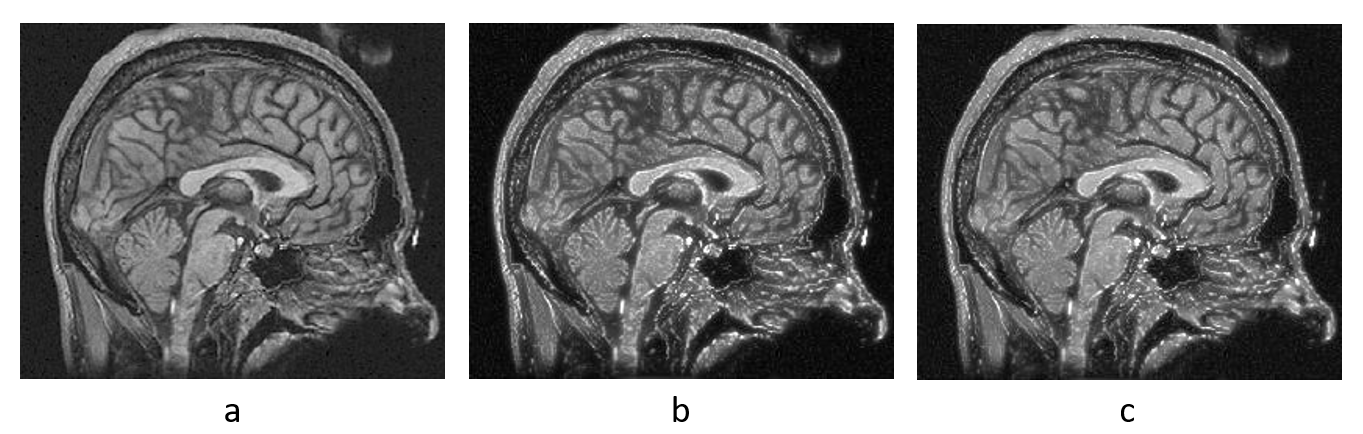
\includegraphics[scale=0.43]{Figures/fig14.png}
    \par \textbf {Hình 2.7} Lọc sắc nét ảnh X-Ray và MRI\\ (a: ảnh gốc, b: Gaussian, c: Butterworth).
\end{center}
Có thể thấy rằng sự tương phản trong ảnh được tăng lên, các đường biên trong ảnh đã được tăng cường và nổi bật hơn so với ảnh gốc. Ảnh chụp X-Ray thân trên của người có các đường biên ở xương sườn, xương cẳng tay, hệ thống mạch phía dưới phổi được kích sáng hơn, dễ dàng nhận diện các khu vực bị gãy, nứt. Ảnh MRI qua phép lọc nổi bật hơn và đồng thời cũng loại bỏ được phần nhiễu xung quanh.
\subsection{Lọc nhiễu ảnh trong nhận dạng vân tay}
Nhận dạng vân tay là một bài toán gặp nhiều khó khăn ở giai đoạn tiền xử lý. Ảnh vân tay thu được thường gặp những vết mờ, bẩn, nhiều nơi đường vân không rõ nét. 
\begin{center}
    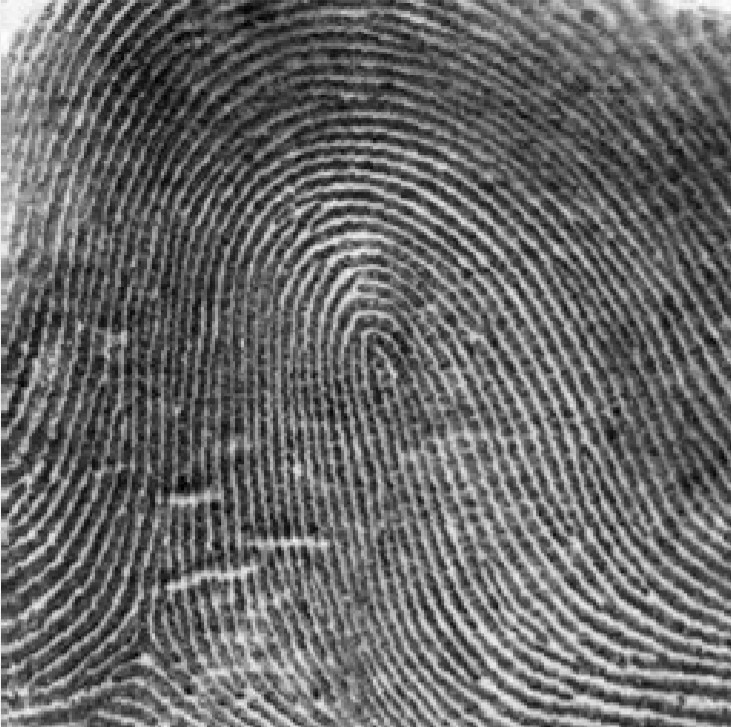
\includegraphics[scale=0.4]{Figures/anh_van_tay.jpg}
    \par \textbf {Hình 2.8} Ảnh mẫu vân tay.
\end{center}
Việc loại bỏ nhiễu có thể thực hiện đơn giản bằng phép lọc thông cao Butterworth, giúp giữ lại chỉ những đặc trưng đường vân quan trọng. Ta thu được kết quả sau khi sử dụng phép lọc thông cao Butterworth cấp 4:
\begin{center}
    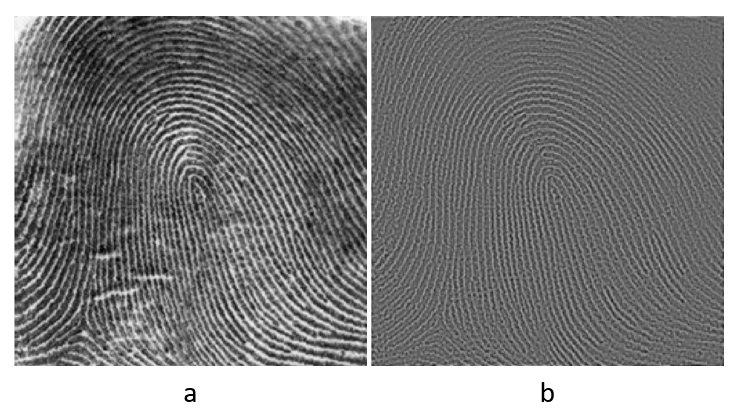
\includegraphics[scale=0.8]{Figures/fig13.png}
    \par \textbf {Hình 2.9} Khử nhiễu mẫu vân tay \\ (a: ảnh gốc, b: ảnh đã tăng cường).
\end{center}
Thông qua ảnh đã được lọc, đặc trưng có thể dễ dàng thu được phục vụ cho mục đích nhận dạng.
\subsection{Khử nhiễu ảnh trong công nghệ OCR}
Trong nền công nghiệp in ấn, đôi khi máy tính phải xử lý những bức ảnh chụp/scan chữ bị nhiễu, nhòe, mờ làm giảm chất lượng hình ảnh và gây khó khăn cho quá trình OCR (nhận diện kí tự quang học - Optical Characters Recognition). Để khắc phục điều này, giai đoạn tiền xử lý là tối quan trọng. Bên cạnh việc sử dụng việc áp dụng linh hoạt các phương pháp lọc, chẳng hạn lọc thông thấp giúp ảnh mượt (hình 2.11), thông qua phép biến đổi tích chập (convolution) và định lý tích chập được đề cập trong phần 1.2.5, các phép lọc ảnh sử dụng tích chập đã được sử dụng một cách phổ biến và linh hoạt, đặc biệt là các phép biến đổi hình học Morphology [16], mang lại nhiều tiện lợi và hiệu quả trong quá trình tiền xử lý hình ảnh.
\begin{center}
    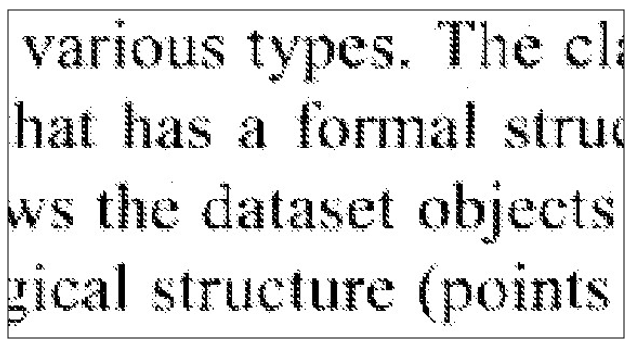
\includegraphics[scale=0.65]{Figures/fig15b.png}
    \par \textbf {Hình 2.10} Ảnh bị lỗi khi scan.
\end{center}
\begin{center}
    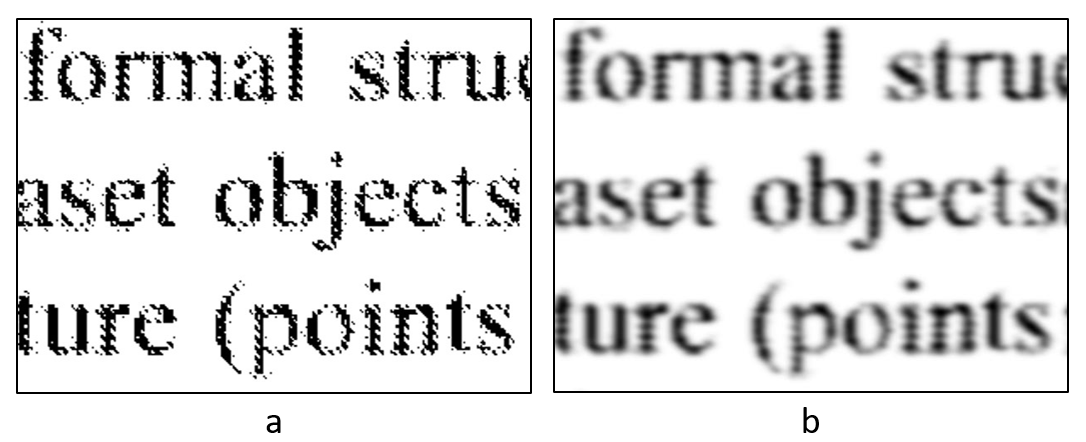
\includegraphics[scale=0.5]{Figures/fig11a.png}
    \par \textbf {Hình 2.11} Làm mượt ảnh trong bài toán OCR \\(a: ảnh nhiễu thu được từ máy in/scan, b: ảnh đã được làm mượt Gaussian).
\end{center}
Ta có thể tiến hành lọc ảnh bằng cách kết hợp nhiều phương pháp.

\begin{lstlisting}[language=Octave]
img = imread('input.png');
% Reverse image
img = 1.0 - double(img)/255.0;
% Create convolution-2D kernels
n = false(3);n(4) = 1;
s = false(3);s(6) = 1;
w = false(3);w(2) = 1;
e = false(3);e(8) = 1;
% Erode Morphology Mixture
fourNeighbourCount = imerode(img,n) + imerode(img,s) + imerode(img,w) + img;
img = fourNeighbourCount > 1;
% Smooth image using Low pass Gaussian
img = real(GaussLowPass(img, 30));
% Reverse again
imwrite(1.0-mat2gray(img), 'path-to-output-directory');
% Define Low-pass Filter Gaussian
function filted_img = GaussLowPass(img, sig)
    fft_img = fftshift(fft2(double(img)));
    [H,W,c] = size(img);
    ctx = (W-1)/2;
    cty = (H-1)/2;
    a = 1/(2*pi*sig*sig);
    b = 2*sig*sig;
    [x, y] = meshgrid(1:W, 1:H);
    D2 = (x - ctx ).^2 + (y - cty).^2;
    filter = a*exp(-D2/b);
    im = zeros(size(img));
    for z = 1:c
        im(:,:,z) = fft_img(:,:,z).*filter;
    end 
    filted_img = ifft2(ifftshift(im));
end
\end{lstlisting}
Bằng việc kết hợp giữa các toán tử biến đổi hình học Morphology (cụ thể trong trường hợp trên là phép lọc Erode [16]) và phép lọc thông thấp Gaussian, ta thu được kết quả tốt hơn so với việc chỉ sử dụng lọc thông thấp:
\begin{center}
    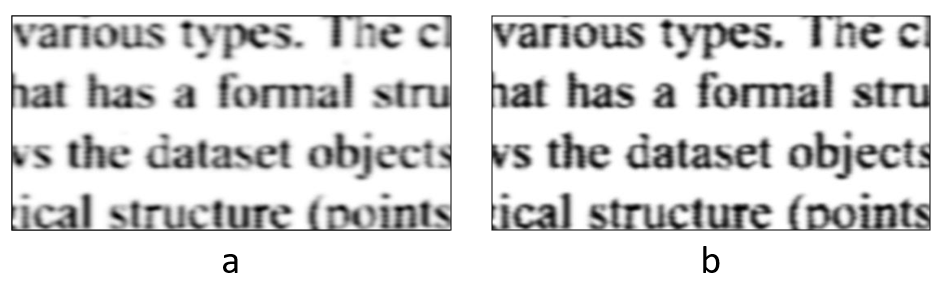
\includegraphics[scale=0.65]{Figures/fig15a.png}
    \par \textbf {Hình 2.12} Làm mượt ảnh trong bài toán OCR \\(a: ảnh được lọc thông thấp Gaussian, b: ảnh được lọc kết hợp).
\end{center}
Bên cạnh đó, phép lọc ngưỡng có thể được áp dụng sau phép lọc thông thấp trong trường hợp nền xung quanh chịu ảnh hưởng bởi nhiễu trong quá trình in ấn:
\begin{center}
    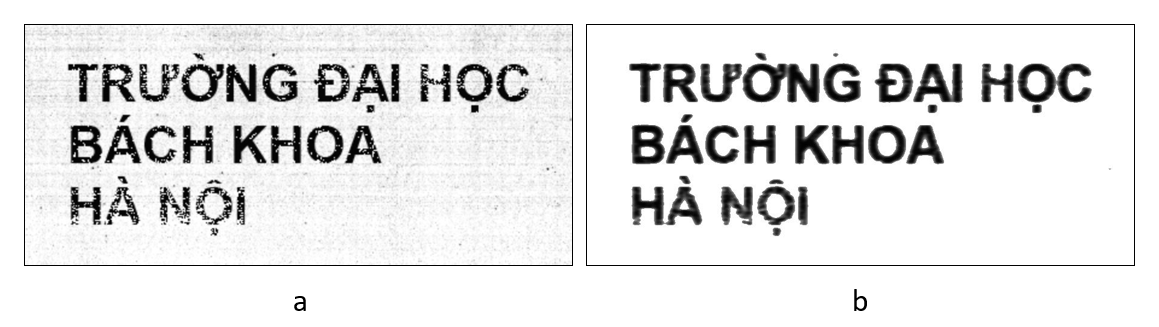
\includegraphics[scale=0.50]{Figures/fig15c.png}
    \par \textbf {Hình 2.13} Làm mượt ảnh trong bài toán OCR \\(a: ảnh gốc, b: ảnh được lọc kết hợp với ngưỡng).
\end{center}
\subsection{Khử răng cưa}
Hiện tượng răng cưa (aliasing) xuất hiện khi ta thực hiện phục hồi ảnh từ ảnh đã thu nhỏ, hay phóng lớn ảnh từ ảnh kích thước nhỏ. Khử răng cưa (anti-aliasing) có thể được thực hiện đơn giản bằng phép làm mượt ảnh:
\begin{center}
    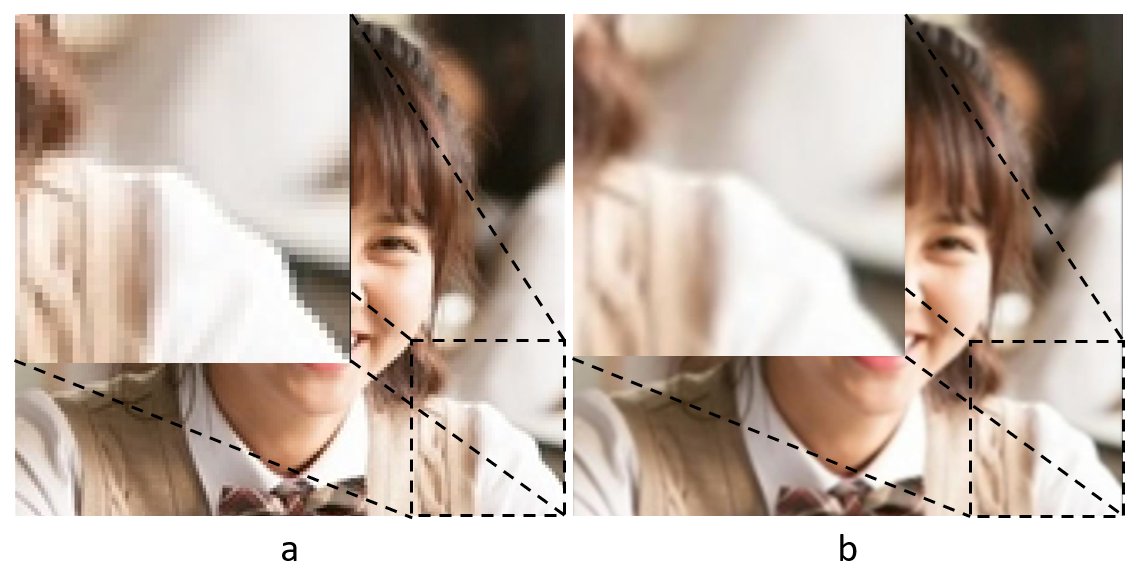
\includegraphics[scale=0.5]{Figures/fig16.png}
    \par \textbf {Hình 2.14} Khử răng cưa trong ảnh \\(a: ảnh bị răng cưa khi phóng lớn, b: ảnh được làm mượt bằng phép lọc Gaussian).
\end{center}